\chapter{Theoretical framework: active suspensions}
\label{active_suspensions}

Active suspensions are densely packed soft materials whose constituents can self-propel.

In turn, soft materials~\cite{Soft_materials} are those that can be easily deformed by external stresses, electric or magnetic fields, or by thermal fluctuations. 

As Pierre-Gilles de Gennes said during his Nobel Prize lecture~\cite{PGG}, another designation for these materials is \textit{complex fluids}, which renders very well their complex and flexible character.

They are considered 'structured fluids' because they have the local mobility of ordinary fluids, but they always show a degree of local order (see~\cite{soft_matter},~\cite{Hamley}).

In particular, we will be working with biological soft materials\footnote{In the introduction we mentioned the existence of synthetic active suspensions. For the sake of brevity, they remain out of the scope of this document. If the reader is curious about this topic, further information can be found, for instance, in the paper of Thutupalli et al.~\cite{Thutupalli}, who experimentally studied the behavior of droplets displacing under Marangoni stresses.} which may, or not, be amphiphile \footnote{Surfactants are amphiphilic compounds: they possess both hydrophilic and hydrophobic moieties (head and tail respectively).} solutions as well.

Contrary to many other soft materials, the presence of \textit{Chlamydomonas reinhardtii} does not seem to affect the rheological properties of water significantly (i.e. it stays a Newtonian fluid with a very similar viscosity coefficient).

Surfactants may, on the other hand, change some of these properties in a local way, mainly at the surfaces (where they are mostly concentrated), as a consequence of the Marangoni effect.

It is though clear that diffusion is modified (enhanced) by the action of \textit{Chlamydomonas reinhardtii}, so the sections hereafter are devoted to biological and physical aspects of this alga.

\section{\textit{Chlamydomonas reinhardtii}}

\subsection{Classification and biological description}

We have already mentioned that \textit{Chlamydomonas reinhardtii}
is a unicellular green alga, but we would like to provide with a more exhaustive description through its taxonomic classification: 

\begin{itemize}
	\item \textbf{Superregnum}: Eukaryota - Organisms whose cells have a nucleus enclosed within membranes	
	\item \textbf{Regnum}: Plantae/Viridiplantae - Clade made up of the green algae, which are primarily aquatic, and the land plants
	\item \textbf{Divisio}: Chlorophyta - Division of the green algae that comprises about 8200 species, the majority of whom are aquatic and photosynthetic
	\item \textbf{Classis}: Chlorophyceae - One of the classes of green algae, distinguished mainly on the basis of ultrastructural\footnote{Ultrastructure is the architecture of cells and biomaterials that is visible at higher magnifications than found on a standard optical light microscope (e.g.: organelles)} morphology
	\item \textbf{Ordo}: Volvocales/Chlamydomonadales~\cite{chlorophyceae} - Members of these orders have a 1 o'clock-7 o'clock arrangement of the basal bodies of the flagella.
	\item \textbf{Familia}: Chlamydomonadaceae - This family includes all the unicellular Volvocales. They may be bi- or quadriflagellate.
	\item \textbf{Genus}: Chlamydomonas\footnote{For further information on the genus Chlamydomonas we recommend the book of Pandey~\cite{Pandey}} - Here are some criteria customarily used to define a genus:
	??? REESCRIBIR ???
		\subitem Monophyly – All descendants of a particular ancestral taxon are ranked together.
		\subitem Reasonable compactness – The characteristics of the descendants should not be expanded too much.
		\subitem Distinctness – Similar DNA sequences, biogeographical features, ecological features and morphological features of the organisms can be used to rank them in a particular genus. One important trait is that they are biflagellated.
	\item \textbf{Species}: Chlamydomonas reinhardtii - according to Pröschold et al.~\cite{Proschold}, all the current “standard” \textit{C. reinhardtii} strains are presumably derived from a single field-isolated zygote in Massachusetts in 1945\footnote{For detailed information, both the article od Pröschold et al. and the one of Harris~\cite{Harris} should be consulted.}. Its diameter is about 10 micrometres; it has a cell wall, a large cup-shaped chloroplast, and an "eyespot" that senses light. 
\end{itemize}

The figure below shows a schematic of the cross section of \textit{C. reinhardtii}:

\begin{figure}[H]
	\centering
	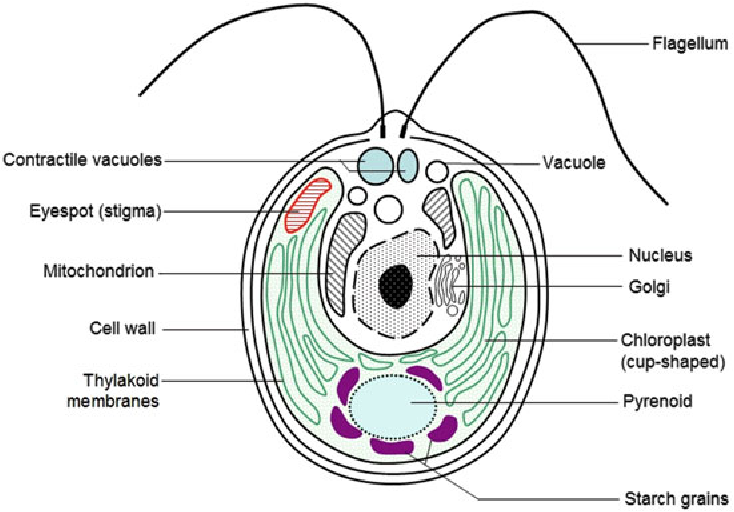
\includegraphics[width=0.8\textwidth]{archivos/chlamy_illustration.png}
	\caption{Schematic of \textit{C. reinhardtii} cross section~\cite{chlamy_cs}
	}
	\label{chlamy_illustration}
\end{figure}

Especially important to our research is the motion of this alga and its mechanisms. A more mechanical point of view will be adopted in the next section, but we consider it important to explain some phenomena that could modify the motion patterns of \textit{C. reinhardtii}. Originated in response to a stimulus, this movements are referred to as taxes. Depending on the cause they are classified as: aerotaxis (stimulation by oxygen), barotaxis (by pressure), chemotaxis (by chemicals), galvanotaxis (by electric current), gravitaxis (by gravity), hydrotaxis (by moisture), magnetotaxis (by magnetic field), phototaxis (by light), rheotaxis (by fluid flow), thermotaxis (by changes in temperature), thigmotaxis (by physical contact)...

Given the low thickness of the films we will be working with, the effects of aerotaxis and gravitaxis should be negligible. A correct mixing of the suspension should prevent chemotaxis as well. Phototaxis and thermotaxis could constitute a problem and oblige to the use of red light when observing the algae. A red filter should also reduce the thermal- and evaporation-induced flows, and thus rheotaxis. To avoid barotaxis and thigmotaxis, the observed area must be far enough from the borders of the domain.

\subsection{Physical description and modelisation}

The study of the motion of microorganisms (microswimmers) in an analytical way was first addressed by Lighthill in 1952~\cite{Lighthill}. He developed the \textit{spherical squirmer model}, which considers the microorgnism as a spherically shaped particle that uses small-amplitude, axisymmetric surface distortions to move through the surrounding fluid.

Still today, the spherical squirmer is widely used as a model for self-propelled particles, such as unicellular protists, algae, Janus particles\footnote{Janus particles are entities whose surface shows different functionalities on different parts of it~\cite{PGG}.}, etc. in Stokes flow.

Later, in 1971, Lighthill’s student John Blake,  corrected and refined Lighthill's theory. This model tackled ciliated organisms and involved the behavior of the envelope covering the end of that cilia. 

\begin{figure}[H]
	\centering
	\includegraphics[width=0.6\textwidth]{archivos/BlakeWave.PNG}
	\caption[Caption for LOF]{Envelope showing a symplectic metachronal wave\protect\footnotemark ($---$)~\cite{Pedley}}
	\label{symplectic_wave}
\end{figure}

As it can be seen on the previous figure, the cilia take on asymmetric conformations to overcome the time reversibility of Stokes flows: during the power stroke they are mostly stretched and during the recovery strokes they remain contracted.

Regarding the spherical simplification, in Blake's own words: \textit{Considering the problem of a sphere is highly idealizing the shape of the organism, but at low Reynolds number the shape does not alter the hydrodynamical features very greatly.} With the right coordinate transformation, other shapes could be considered, but it would add nothing new beyond making the calculations more obscure.

\footnotetext{A phase difference between the flagella leads to the generation of a metachronal wave. A negative phase difference creates symplectic waves (i.e. the direction of beat and wave transmission is the same) due to compression of the cilia during the effective stroke phase. A positive phase difference results in antiplectic waves (i.e. the directions of beat and wave transmission are opposed) by compression on the cilia during the recovery stroke.}

In the considered case (low $Re$, incompressible, axisymmetric flow), the equations of motion for the velocity $\mathbf{u}$ and pressure $p$ are: 

\begin{equation}
\begin{aligned} & \nabla \cdot \mathbf{u}=0 \\
& \nabla p-\mu \nabla^{2} \mathbf{u}=\mathbf{F} \label{stokes_f} \end{aligned}
\end{equation}

It is clear, that, due mainly to its tiny size and relatively low speed, microorganisms live in the world of low Reynolds number. However, for this equations to be adapted, another condition must be accomplished since swimming flows are usually unsteady: the ‘frequency Reynolds number’ $Sr \cdot Re = \rho \omega l_c^2/ \mu_g$ (where $Sr$ is the Strouhal number) must also be small.

In our problem the value of both Reynolds numbers can be estimated as follows:

\begin{equation}
	\begin{aligned} & Re = \rho_g u_c l_c/\mu_g \simeq 1.32 \cdot 10^{-4} << 1\\
	& Sr \cdot Re = \rho_g \omega_cl_c^2/ \mu_g \simeq 4.96 \cdot 10^{-4} << 1 \end{aligned}
\end{equation}

as $\rho_p = 1.05 \; \textrm{g/} \textrm{cm}^\textrm{3}$, $l_c = 1 \; \mu \textrm{m}$,  $u_c = 100 \; \mu \textrm{m/s}$,  $\omega_c = 2 \pi 60 \; \textrm{rad/s}$, and we consider the worst-case scenario regarding the temperature: $\mu_g(30^\textrm{o}\textrm{C}) = 7.98 \cdot 10^{-4} \; \textrm{kg/(m} \cdot \textrm{s)}$

These values widely justify the use of the Stokes equations in this context.

A very interesting interpretation of the Reynolds number is provided by Lauga and Powers in their 2009 article on \textit{The hydrodynamics of swimming microorganisms}~\cite{Lauga}. The Reynolds number would compare the time scales for the convective transport of a local velocity perturbation along the body ($t_{adv} \sim l_c/u_c$), and for viscosity to diffuse this perturbation  away from the body ($t_{diff} \sim ρl_c^2/ \mu_g$). 

As a consequence, in low Reynolds number flows, velocity perturbations diffuse before being carried along by the flow and thus the response of the fluid to the displacement of its boundaries must be immediate. 

In conclusion, the acceleration of a microswimmer is negligible as against the forces from the surrounding fluid. As a result of this absence of inertia, Newton’s law becomes:

\begin{equation}
\mathbf{F_{\mathrm{ext}}}(t)+\mathbf{F}(t)= \mathbf{0}
\end{equation}

which constitutes an instantaneous balance between external and fluid forces \footnote{A similar result can be found regarding the torques, but we will not make use of it in this document.}.

Consequently, in absence of external forces $\mathbf{F}(t) = \mathbf{0}$. This obviously requires a density matching of the swimmers and the medium.

Equations \ref{stokes_f} become then:

\begin{equation}
\begin{aligned} & \nabla \cdot \mathbf{u}=0 \\
& \nabla p-\mu \nabla^{2} \mathbf{u}=\mathbf{0} \label{stokes_f} \end{aligned}
\end{equation}

Since only motions with axial symmetry are considered, spherical polar co-ordinates represent a logical choice. With a moving origin that remains at the center of the body \footnote{Lighthill justifies neglecting any inertial translation this origin may undergo because: \textit{This motion of the origin makes no difference to the equations of motion, since the inertial force associated with it is clearly equally negligible with those already neglected.}}, the solution in terms of radial and azimuthal velocities $u_r$ and $u_\theta$ presented by Blake~\cite{Blake} is:

\begin{equation}
\begin{aligned} u_{r}\left(r, \theta_{0}\right)=&-U \cos \theta_{0}+A_{0} \frac{a^{2}}{r^{2}} P_{0}+\frac{2}{3}\left(A_{1}+B_{1}\right) \frac{a^{3}}{r^{3}} P_{1} \\ &+\sum_{n=2}^{\infty}\left[\left(\frac{1}{2} n \frac{a^{n}}{r^{n}}-\left(\frac{1}{2} n-1\right) \frac{a^{n+2}}{r^{n+2}}\right) A_{n} P_{n}+\left(\frac{a^{n+2}}{r^{n+2}}-\frac{a^{n}}{r^{n}}\right) B_{n} P_{n}\right] \\ u_{\theta}\left(r, \theta_{0}\right)=& U \sin \theta_{0}+\frac{1}{3}\left(A_{1}+B_{1}\right) \frac{a^{3}}{r^{3}} V_{1} \\+& \sum_{n=2}^{\infty}\left[\left(\frac{1}{2} n \frac{a^{n+2}}{r^{n+2}}-\left(\frac{1}{2} n-1\right) \frac{a^{n}}{r^{n}}\right) B_{n} V_{n}+\frac{1}{2} n\left(\frac{1}{2} n-1\right)\left(\frac{a^{n}}{r^{n}}-\frac{a^{n+2}}{r^{n+2}}\right) A_{n} V_{n}\right] \end{aligned}
\label{stokes_sol_uv}
\end{equation}

where $a$ is the radius of the spherical squirmer, $B_n$ are constant coefficients, $P_n(cos \theta)$ are Legendre polynomials\footnote{Solutions to the Legendre Differential Equation, whose form is:\\ $P_{n}(x)=\sum_{m=0}^{M}(-1)^{m} \frac{(2 n-2 m) !}{2^{n} m !(n-m) !(n-2 m) !} x^{n-2 m}$ with \\ $M=n / 2$ or $(n-1) / 2,$ whichever is an integer} and:

\begin{equation}
V_{n}(\cos \theta)=\frac{2}{n(n+1)} P^1_{n}(\cos \theta)
\end{equation}

where $P^1_n$ is the associated Legendre function of the first kind\footnote{The defining relationship between Legendre functions (of order $m$) and Legendre polynomials is: $P_{n}^{m}(x)=\left(1-x^{2}\right)^{m / 2} \frac{d^{m} P_{n}(x)}{d x^{m}}$}.

The coefficients of \ref{stokes_sol_uv} correspond to the sole solution that fulfills the boundary conditions at the surface\footnote{The boundary conditions are given at $r=a$ because the amplitude of the perturbations is much smaller than $a$} of the squirmer:

\begin{equation}
u_r|_{r-a}=\sum_{0}^{\infty} A_{n} P_{n}, \quad u_\theta|_{r-a}=\sum_{0}^{\infty} B_{n} V_{n}
\end{equation}

Among the fundamental solutions that conform \ref{stokes_sol_uv} we must only retain those which represent motions with a finite total energy (infinite energy solutions can only arise of the continued application of an external force). As a consequence, to avoid infinite terms resulting from the integration leading to the system's energy, the velocity of the origin must be:

\begin{equation}
	U=\frac{1}{3}\left(2 B_{1}-A_{1}\right)
	\label{deformation_vel}
\end{equation}

This condition also requires to omit the \textbf{Stokeslet} term ($\propto r^{-1}$ in 3D) in both expressions (it has been already omitted in Eqs.\ref{stokes_sol_uv}), meaning that the Stresslet solution ($\propto r^{-2}$ in 3D)\footnote{Stresslets are obtained by differentiation of the Stokeslets and, thus, their spatial decay is faster.} will dominate the field.

With the aim of illustrating the fundamental solutions to the Stokes equation, Fig. \ref{stokeslet_stresslet} shows the velocity field corresponding to a Stokeslet and a Stresslet in 3D.

\begin{figure}[H]
	\centering
	\includegraphics[width=0.8\textwidth]{archivos/stokesletstresslet.jpg}
	\caption{Velocity field around a Stokeslet (left) and around a Stresslet (left)~\cite{Singh2015}. Streamlines are overlaid on a pseudocolor plot of the logarithm of the magnitude of the fluid velocity in a planes containing the axis of the symmetry}
	\label{stokeslet_stresslet}
\end{figure}

Another point of view that would equally lead us to omit the Stokeslet term is the fact that these solutions are associated with singular point forces, which, as we have already explained, are not present in this problem. 

The given explanation, however, is not trivial and it can help to look at a smaller scale of our specific problem, where one can consider two Stokelet fields that somehow compensate each other: the flagellar thrust and the body drag~\cite{Lokenath}. In their 2018 paper~\cite{Drescher2010}, Drescher et al. develop a three-Stokeslet model that illustrates this thrust-drag balance (see Fig. \ref{drag_thrust}).

\begin{figure}[H]
	\centering
	\includegraphics[width=0.7\textwidth]{archivos/velfield.png}
	\caption{Time- and azimuthally- averaged flow field of \textit{C. reinhardtii}. (a) Streamlines (red) computed from velocity vectors (blue). The spiraling near elliptic points is an artifact of the direct integration a noisy experimental velocity field. A color scheme indicates flow speed magnitudes. (b) Streamlines of the azimuthally averaged flow of the three-Stokeslet model: flagellar thrust is distributed among two Stokeslets placed (not fitted) at the approximate flagellar position (lateral green arrows), whose sum balances drag on the cell body (central red arrow)~\cite{Drescher2010}.}
	\label{drag_thrust}
\end{figure}

Finally one can derive an expression for the pressure:

\begin{equation}
p=\mu_{n=2}^{\infty} \frac{2 n-1}{n+1}\left(n A_{n}-2 B_{n}\right) \frac{a^{n}}{r^{n+1}} P_{n}\left(\cos \theta_{0}\right)
\end{equation}

The fact that flagella and cilia, although similar, show some important differences cannot be ignored. Nonetheless, the squirmer model remains applicable.

Extensions to ellipsoidal swimmers and time-dependent swimming gaits for a reduced squirmer model are explained in Delmotte  et al.~\cite{Delmotte2015}. Although the time-averaged models (e.g.: squirmer model with constant coefficients) provide with valid results for the far field, the experimental works of Guasto et al.~\cite{Guasto} suggest that time dependence has, in fact, an important effect on the close field of a swimmer. This must be taken into account when working with high swimmer concentrations.

The reduced model used by Delmotte is proposed by Ishikawa et al. in~\cite{Ishikawa}. It considers $A_n=0$ for all $n$ and $B_n=0$ for all $n >2$. The resulting flow field in the moving frame attached to the swimmer is:

\begin{equation}
\begin{array}{l}{\mathbf{u}_{\Gamma}(r, \theta)=\frac{2}{3} B_{1} \frac{a^{3}}{r^{3}} P_{1}(\cos \theta)+\left(\frac{a^{4}}{r^{4}}-\frac{a^{2}}{r^{2}}\right) B_{2} P_{2}(\cos \theta)} \\ {\mathbf{u}_{\theta}(r, \theta)=\frac{1}{3} B_{1} \frac{a^{3}}{r^{3}} V_{1}(\cos \theta)+\frac{a^{4}}{r^{4}} B_{2} V_{2}(\cos \theta)}\end{array}
\end{equation}

In the absence of $A_1$, Eq. \ref{deformation_vel} shows that the first mode and, thus, $B_1$ is directly related to the swimming speed. It can also be shown [28] that the second mode and its coefficient, $B_2$, are directly related to the Stresslet. 

A parameter $\beta=B_2/B_1$ can now be introduced that describes the relative Stresslet strength and allows us to distinguish two sorts of mechanisms: when $\beta>0$, the squirmer behaves like a \textit{puller}, bringing fluid in along its swimming direction and expelling it laterally; otherwise ($\beta<0$), the squirmer acts like a \textit{pusher}, expelling fluid along  its swimming direction and bringing it in laterally. Examples of the flow patterns induced by this two types of microswimmers can be observed in Fig. \ref{push_pull}.

\begin{figure}[H]
	\centering
	\includegraphics[width=0.6\textwidth]{archivos/push_pull.png}
	\caption{Schematics showing the flow patterns induced by classical (a) pushers (\textit{Escherichia coli}) and (b) pullers (\textit{Chlamydomonas reinhardtii}). The color indicates the magnitude of the flow ($r^{−2}$ scaling because of the dominating Stresslet).~\cite{Yang}}
	\label{push_pull}
\end{figure}

On one hand, \textit{Pushers} and \textit{pullers} show some differences regarding the rheological properties of the suspension they are immersed in: the effective viscosity is increased in the case of \textit{pullers} and decreased for \textit{pushers}.

On the other hand, the enhancement of diffusion or mixing has very similar characteristics, that will be discussed in greater depth in the State of the art section. 